\chapter{概要设计}

本节描述系统的概要设计过程以及系统概要设计。课程管理系统的设计与办公自动化(Office Automation, OA)系统同为面向业务的应用拥有很多相似的设计,本项目在设计上也参考了典型的 OA 系统设计模式,同时借鉴 RIA 系统的设计思想,使项目既能保持业务的高度一致性,又能应对开发过程中所发生的各类变更。

\section{体系结构设计}

图~\ref{Architecture} 简单描述了系统的基础架构。

\begin{figure}[!h]
  \begin{center}
    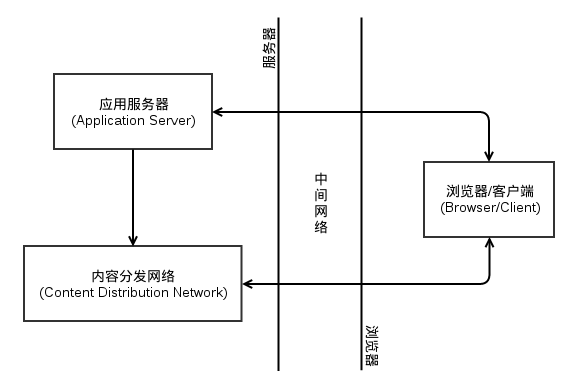
\includegraphics[scale=0.5]{figures/diagram-architecture.png}
    \caption{系统架构示意图\label{Architecture}}
  \end{center}
\end{figure}

基于经典的 Client/Server (C/S) 架构模式。在 C/S 模式的基础上,基于浏览器这一特殊的执行环境(Execution Context),客户端程序并不直接部署在用户终端上,架构中加入了内容分发网络用于分发静态的客户端程序数据。

接下来,与现在典型的 MVVM 应用方式不同\footnote{Angular.js、Knockout.js等流行的JavaScript实现将MVVM作为客户端框架进行实现},我们在C/S的基础架构上,应用MVVM架构(图~\ref{ArchitectureMVVM})

\begin{figure}[!h]
  \begin{center}
    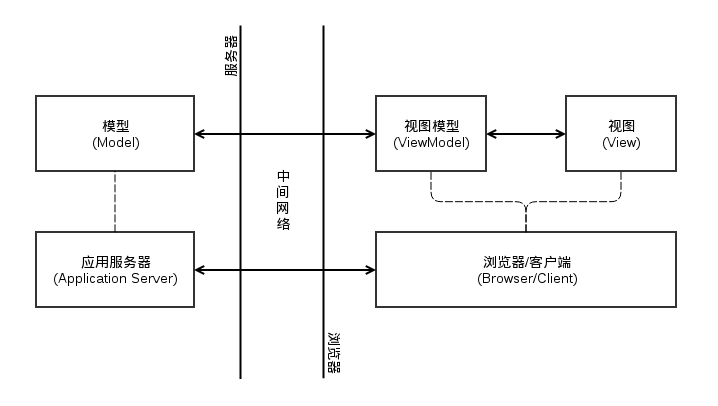
\includegraphics[scale=0.5]{figures/diagram-architecture-mvvm.png}
    \caption{MVVM 系统架构示意图\label{ArchitectureMVVM}}
  \end{center}
\end{figure}

服务器提供MVVM框架中模型(Model)的支持,负责响应业务请求和维护业务数据,客户端提供视图(View)以及视图模型(ViewModel)负责业务数据的呈现逻辑和用户事件的处理\footnote{服务器与客户端之间的通信属于ViewModel的一部分}。

下面将分两个小节分别介绍服务器和客户端的二级架构方案。

\subsection{服务器架构方案}

将服务器部分作为Model进行设计的一大特点是服务器设计的轻量化,这与常见的RIA应用中的服务器设计是基本相符的,服务器为业务数据共享、权限管理等基本需求提供了支持。

\begin{figure}[!h]
  \begin{center}
    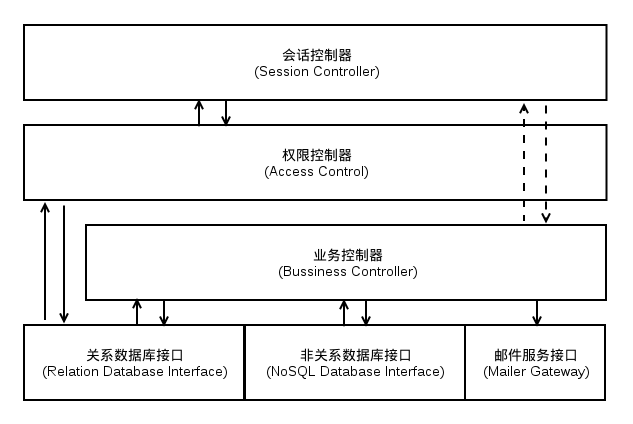
\includegraphics[scale=0.5]{figures/diagram-architecture-server.png}
    \caption{服务器架构示意图\label{ArchitectureServer}}
  \end{center}
\end{figure}

图~\ref{ArchitectureServer} 说明服务器的分层架构模式:

\begin{itemize}
  \item 顶层通过 HTTP/HTTPS 提供的会话层对会话状态进行管理
  \item 权限控制器提供账户服务
  \begin{itemize}
    \item 处理账户登录、注册等账户相关数据业务
    \item 拒绝超出权限范围的访问请求、保障用户逻辑输入的正确性
    \item 向业务逻辑层提供透明的用户认证机制
  \end{itemize}
  \item 业务逻辑层实现产生商业价值的业务逻辑
  \item 最下层为数据持久化以及外部服务层
\end{itemize}

服务器利用混合数据库模式,关系型数据库管理业务数据等强关系关联的数据、非关系型数据库处理会话数据等弱关系数据。(见~\ref{sec:Database})

\subsection{客户端架构方案}

上文中提到客户端实现整体架构中的View以及ViewModel部分

\begin{figure}[!h]
  \begin{center}
    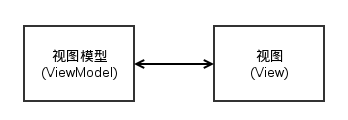
\includegraphics[scale=0.5]{figures/diagram-architecture-client.png}
    \caption{客户端架构示意图\label{ArchitectureClient}}
  \end{center}
\end{figure}

视图 (View) 在系统中被定义为一系列模板的集合,ViewModel 处理页面逻辑,经典 MVVM 模式当中的 DataBinding 模式由特殊的 ViewModel 实现。

\section{数据库设计\label{sec:Database}}

本项目主要使用关系型数据库系统(Relational Database System, RDBS)进行业务数据的管理。

在面向业务的系统构建,特别是 MVVM 模式构建的系统当中,对数据的清晰定义将影响到系统业务的稳定性、可靠性、可扩展性等多个重要的性能。定义良好的数据规格可以直接成为 MVVM 模式中 Model 定义的来源。

本节首先描述课程管理系统数据库的设计概要以及一些需要特别说明的设计概念,后面几个小节描述课程数据、表单数据、用户数据模型的设计方案。

\newpage

\subsection{数据库设计概要}

下图简单的列出了数据库设计(详见~\nameref{sec:appendix-database-diagram})

\begin{figure}[!h]
  \begin{center}
    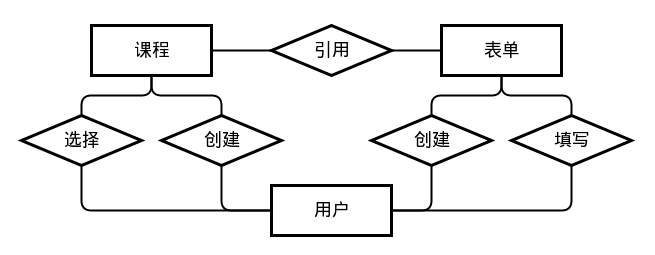
\includegraphics[scale=0.5]{figures/diagram-er-overview.png}
    \caption{数据库E-R关系示意图\label{DatabaseOverview}}
  \end{center}
\end{figure}

系统主要有下面三类业务数据实体:

\begin{itemize}
  \item 课程数据实体
  \item 表单数据实体
  \item 用户数据实体
\end{itemize}

需要特别说明的是 \textbf{表单数据实体} 用于存储系统内其他实体所引用的表单定义。在现实的业务交往过程当中,业务的完成流程往往是基于表格的,创建业务管理系统的核心就在于对表单的创建、维护以及对填写好的表单进行归档、整理。因此,在系统的设计过程中通过创建通用的表单数据实体,将业务数据需求通过表单数据实体进行描述,能避免系统内对业务数据的检索,提高数据库的可扩展性以及系统的业务灵活度。

同时,系统内存在下面业务关系:

\begin{itemize}
  \item 选课业务关联
  \item 表单引用关联
  \item 标签/域关联~\footnote{为了让图形语言表达更清晰,本关联未在图~\ref{DatabaseOverview} 中得到体现。}
  \item 创建者关联
\end{itemize}

\textbf{标签/域关联} 是为了满足系统对系统内数据实体访问权限的细化控制需求而设定的配置数据,这是一组在所有实体上都可以实现的“接口”,实体通过限定“域(Scope)”确定有权限访问该实体的“标签(Tag)”。标签是对“搜索”逻辑的简化和抽象,使用标签机制可以更高效地完成对数据实体的筛选操作,基于标签的检索也能够更有效的保证数据库系统的安全性与可靠性。

\newpage

\subsection{课程实体设计}

课程实体由导师创建,用于存放课程业务数据,与表单数据之间有紧密的业务联系。

\begin{figure}[!h]
  \begin{center}
    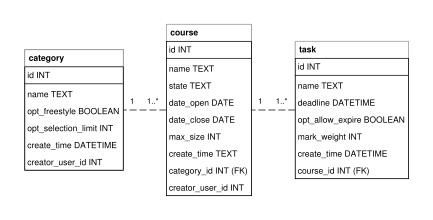
\includegraphics[width=\textwidth]{figures/diagram-eer-course.pdf}
    \caption{课程实体\label{DatabaseEntityCourse}}
  \end{center}
\end{figure}

\textbf{课程(course)} 是与课程管理系统的核心实体,包含了课程的基本信息。

\textbf{任务(task)} 为导师规划课程进展、检测教学成果提供了条件:

\begin{itemize}
  \item 系统可以借助评分权重和每一项任务的评分辅助导师给出学员的课程成绩。

  \item 任务表单由导师维护,添加任务时选取,学生应在截止时间内填写完成表单(作业)并提交,供导师查阅后给出评分。

  \item 任务截止之前(允许超时提交的情况下也包括截止之后)学员可多次提交更新。
\end{itemize}

\textbf{课类(category)} 的设计是为了解决更复杂的选课管理需求:

\begin{itemize}
  \item 课类为每门课程提供一份模板,课类下属的课程需“继承”自该课类(课程类目)
  \item 可由导师定义课类内的选课方案~\footnote{比如,“2010级企业实习实训”课类下,定义每名学员只能选取单一课程,在此课类下创建相关的实习实训职位,自主实习的学生可向负责导师申请添加新的职位信息,导师批准后即给与选取。}
  \item 开放学员选题的课类可由学员向指定导师提交课题,课题信息经过导师审核,经指定导师同意后加入课类
\end{itemize}

\newpage

\subsection{用户/账户实体设计}

用户账户实体存储了用户信息、用户权限等信息,应用层权限控制提供了存储条件。

\begin{figure}[!h]
  \begin{center}
    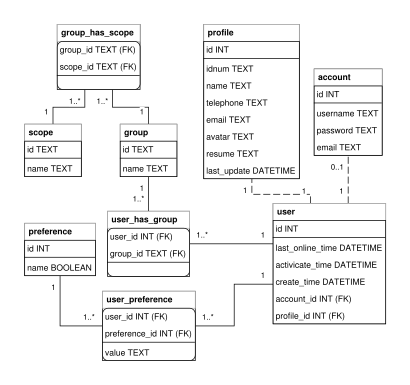
\includegraphics[width=\textwidth]{figures/diagram-eer-user.pdf}
    \caption{用户/账户实体\label{DatabaseEntityUser}}
  \end{center}
\end{figure}

用户在系统内的活动以~\textbf{用户(User)} 实体作为身份标识,\textbf{账户(Account)} 为需要连接的外部身份提供存储支持(如 OpenID 服务)。

数据库配置了基于用户-组-权限的数据结构以存储权限配置,有关权限控制的更多细节请参考~\ref{sec:ServerAPI}。

\newpage

\subsection{表单实体设计}

通过将业务类数据表抽象为表单实体增强了数据库的业务扩展性,减小了数据库和服务器的编码复杂度。

\begin{figure}[!h]
  \begin{center}
    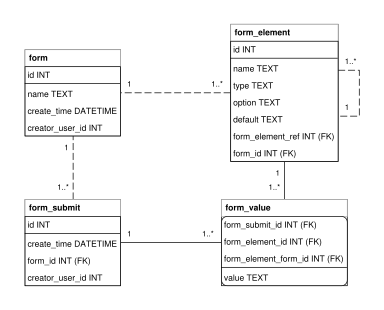
\includegraphics[width=\textwidth]{figures/diagram-eer-form.pdf}
    \caption{表单实体\label{DatabaseEntityForm}}
  \end{center}
\end{figure}

表单项(Form Element) 有如下几种类型~\footnote{表单项类型为类型标识符字符串,由应用逻辑定义并进行解释,数据库仅存储类型标识符与字符串值。}:

\begin{itemize}
  \item 隐藏域(Hidden)
  \item 文本域(Text Input)
  \item 文件域(File)
  \item 图片域(Image)
  \item 地址域(Address/Location)
  \item 单选域(Radio)
  \item 多选域(Checkbox)
  \item 长文本域(Text Area)
  \item 富文本域(Markdown)
  \item 日期域(Date)
  \item 时间域(Time)
  \item 日期/时间(DateTime)
  \item 音频(Audio)
  \item 视频(Video)
  \item 用户(User)
\end{itemize}

值得注意的是 $form\_element$ 定义中包含到 $form\_element$ 的外键用于处理 CheckBox、RadioBox、Selector 等的数据源请求。

\subsection{标签/域模式}

为了解决一系列实体的“搜索”问题(如可见性控制、批量操作),设计标签(Tag)机制给每个可检索实体赋予一组标签。

\begin{figure}[!h]
  \begin{center}
    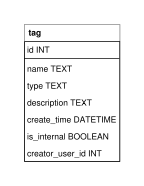
\includegraphics[scale=1.3]{figures/diagram-eer-tag.pdf}
    \caption{标签实体\label{DatabaseEntityTag}}
  \end{center}
\end{figure}

为实体赋予标签需要在实体与标签之间建立多对多的关系,实体的标签能够通过实体的创建者以及管理员进行维护。

实体也能够通过标签进行有效性验证,通过与标签建立多对多的 $filtering$ 关系即可存储有效性验证数据。

\newpage

\section{服务器接口设计\label{sec:ServerAPI}}

服务器接口(通信协议)基于 REST(Representational State Transfer) 服务风格设计~\cite{fielding2002principled}。

\begin{table}[!h]
  \begin{center}
    \noindent
    \ttfamily
    \begin{tabular}{|c|c|l|}
      \hline
      \textbf{符号} & \textbf{资源名} & \textbf{描述} \\ \hline
      u & user      & 用户          \\ \hline
      p & profile   & 用户资料      \\ \hline
      m & message   & 消息          \\ \hline
      g & group     & 课程组(分类)  \\ \hline
      c & course    & 课程          \\ \hline
      t & task      & 任务          \\ \hline
      f & form      & 表单          \\ \hline
      s & submit    & 提交(填表)    \\ \hline
      a & answer    & 答案(任务提交)\\ \hline
      r & review    & 评价(评分)    \\ \hline
      y & registry  & 注册(选课记录)\\ \hline
      e & session   & 会话          \\ \hline
    \end{tabular}
    \caption{URI符号表\label{APURIGlossary}}
  \end{center}
\end{table}

\LTXtable{\linewidth}{parts/table/protocol.tex}

上面的表格给出了服务器开放访问的所有数据资源接口以及接口对访问权限的限制,可以看出通过使用 RESTful 的 API 设计风格,通信协议设计可直接对应参照数据库内的实体设计方法,表~\ref{APURIRelation} 给出的接口之间的关系也对应于数据库实体间的关系。

\begin{table}[!h]
  \begin{center}
    \noindent
    \ttfamily
    \begin{tabular}{|c|l|}
      \hline
      \textbf{符号} & \textbf{资源关系描述} \\ \hline
      (u)/(p) & 用户资料     \\ \hline
      (u)/(m) & 用户消息     \\ \hline
      (u)/(c) & 用户的课程   \\ \hline
      (c)/(m) & 课程消息     \\ \hline
      (c)/(t) & 课程任务     \\ \hline
      (f)/(s) & 表单提交     \\ \hline
      (t)/(a) & 任务答案     \\ \hline
      (a)/(r) & 答案评价     \\ \hline
      (c)/(y) & 课程注册申请 \\ \hline
      (y)/(r) & 课程评价     \\ \hline
      (a)-(s) & 答案引用提交 \\ \hline
      (t)-(f) & 任务引用表单 \\ \hline
      (c)-(g) & 课程引用课类 \\ \hline
      (g)-(f) & 课类引用表单 \\ \hline
    \end{tabular}
    \caption{资源关系表\label{APURIRelation}}
  \end{center}
\end{table}

另外,客户端在访问服务器枚举接口时服务器返回列表内元素的 $id$ 列表,客户端需要对每个元素进行单独访问,这要求客户端有一定的缓存机制作为支持以提升请求性能(或者浏览器支持 HTTP Pipelining 机制)。

\newpage

\section{小结}

本章描述了项目中基于用户需求所进行的系统设计活动:

在系统的体系结构设计当中引入了跨服务器-客户端的 MVVM 模式、确定了轻量服务器的构建模式。

数据库设计遵循关系型数据库设计范式,在保证业务高效和数据一致的前提下为应用层提供了良好的数据可扩展性。

使用 REST 风格制定的服务器接口与数据库设计呈现出高度的一致性。

下一章节将对 ViewModel 与 FRP 做出详细的讨论,导出在对交互实现起到重大作用的 ViewModel 构建方式。

